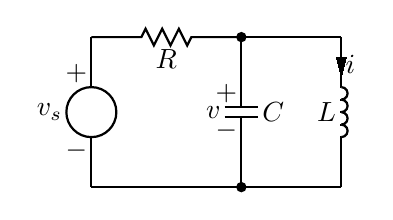
\begin{tikzpicture}[scale=2.54]%
% dpic version 2022.12.01 option -g for TikZ and PGF 1.01
\ifx\dpiclw\undefined\newdimen\dpiclw\fi
\global\def\dpicdraw{\draw[line width=\dpiclw]}
\global\def\dpicstop{;}
\dpiclw=0.8bp
\dpiclw=0.8bp
\dpicdraw (0,0)
 --(0,0.25)\dpicstop
\dpicdraw (0,0.375) circle (0.049213in)\dpicstop
\dpicdraw (0,0.5)
 --(0,0.75)\dpicstop
\draw (0,0.25) node[below left=-2bp]{$ -$};
\draw (-0.125,0.375) node[left=-2bp]{$ v_s$};
\draw (0,0.5) node[above left=-2bp]{$ +$};
\dpicdraw (0,0.75)
 --(0.25,0.75)
 --(0.270833,0.791667)
 --(0.3125,0.708333)
 --(0.354167,0.791667)
 --(0.395833,0.708333)
 --(0.4375,0.791667)
 --(0.479167,0.708333)
 --(0.5,0.75)
 --(0.75,0.75)\dpicstop
\draw (0.375,0.708333) node[below=-2bp]{$ R$};
\dpicdraw[fill=black](0.75,0.75) circle (0.007874in)\dpicstop
\dpicdraw (0.75,0.75)
 --(0.75,0.4)\dpicstop
\dpicdraw (0.666667,0.4)
 --(0.833333,0.4)\dpicstop
\dpicdraw (0.666667,0.35)
 --(0.833333,0.35)\dpicstop
\dpicdraw (0.75,0.35)
 --(0.75,0)\dpicstop
\draw (0.75,0.4) node[above left=-2bp]{$ +$};
\draw (0.666667,0.375) node[left=-2bp]{$ v$};
\draw (0.75,0.35) node[below left=-2bp]{$ -$};
\draw (0.833333,0.375) node[right=-2bp]{$ C$};
\dpicdraw[fill=black](0.75,0) circle (0.007874in)\dpicstop
\dpicdraw (0.75,0.75)
 --(1.25,0.75)\dpicstop
\dpicdraw (1.25,0.75)
 --(1.25,0.5)\dpicstop
\dpicdraw (1.25,0.5)
 --(1.244444,0.5)\dpicstop
\dpicdraw (1.25,0.5)
 ..controls (1.261165,0.5) and (1.271481,0.494044)
 ..(1.277063,0.484375)
 ..controls (1.282646,0.474706) and (1.282646,0.462794)
 ..(1.277063,0.453125)
 ..controls (1.271481,0.443456) and (1.261165,0.4375)
 ..(1.25,0.4375)\dpicstop
\dpicdraw (1.25,0.4375)
 --(1.244444,0.4375)\dpicstop
\dpicdraw (1.25,0.4375)
 ..controls (1.261165,0.4375) and (1.271481,0.431544)
 ..(1.277063,0.421875)
 ..controls (1.282646,0.412206) and (1.282646,0.400294)
 ..(1.277063,0.390625)
 ..controls (1.271481,0.380956) and (1.261165,0.375)
 ..(1.25,0.375)\dpicstop
\dpicdraw (1.25,0.375)
 --(1.244444,0.375)\dpicstop
\dpicdraw (1.25,0.375)
 ..controls (1.261165,0.375) and (1.271481,0.369044)
 ..(1.277063,0.359375)
 ..controls (1.282646,0.349706) and (1.282646,0.337794)
 ..(1.277063,0.328125)
 ..controls (1.271481,0.318456) and (1.261165,0.3125)
 ..(1.25,0.3125)\dpicstop
\dpicdraw (1.25,0.3125)
 --(1.244444,0.3125)\dpicstop
\dpicdraw (1.25,0.3125)
 ..controls (1.261165,0.3125) and (1.271481,0.306544)
 ..(1.277063,0.296875)
 ..controls (1.282646,0.287206) and (1.282646,0.275294)
 ..(1.277063,0.265625)
 ..controls (1.271481,0.255956) and (1.261165,0.25)
 ..(1.25,0.25)\dpicstop
\dpicdraw (1.25,0.25)
 --(1.244444,0.25)\dpicstop
\dpicdraw (1.25,0.25)
 --(1.25,0)\dpicstop
\draw (1.244444,0.375) node[left=-2bp]{$ L$};
\filldraw[line width=0bp](1.225,0.65)
 --(1.25,0.55)
 --(1.275,0.65) --cycle\dpicstop
\dpicdraw (1.25,0.572906)
 --(1.25,0.65)\dpicstop
\draw (1.25,0.611453) node[right=-2bp]{$ i$};
\dpicdraw (1.25,0)
 --(0,0)\dpicstop
\end{tikzpicture}%
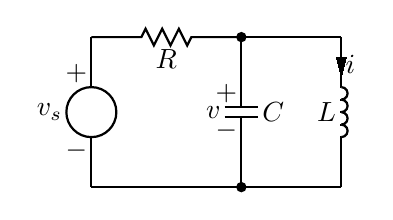
\begin{tikzpicture}[scale=2.54]%
% dpic version 2022.12.01 option -g for TikZ and PGF 1.01
\ifx\dpiclw\undefined\newdimen\dpiclw\fi
\global\def\dpicdraw{\draw[line width=\dpiclw]}
\global\def\dpicstop{;}
\dpiclw=0.8bp
\dpiclw=0.8bp
\dpicdraw (0,0)
 --(0,0.25)\dpicstop
\dpicdraw (0,0.375) circle (0.049213in)\dpicstop
\dpicdraw (0,0.5)
 --(0,0.75)\dpicstop
\draw (0,0.25) node[below left=-2bp]{$ -$};
\draw (-0.125,0.375) node[left=-2bp]{$ v_s$};
\draw (0,0.5) node[above left=-2bp]{$ +$};
\dpicdraw (0,0.75)
 --(0.25,0.75)
 --(0.270833,0.791667)
 --(0.3125,0.708333)
 --(0.354167,0.791667)
 --(0.395833,0.708333)
 --(0.4375,0.791667)
 --(0.479167,0.708333)
 --(0.5,0.75)
 --(0.75,0.75)\dpicstop
\draw (0.375,0.708333) node[below=-2bp]{$ R$};
\dpicdraw[fill=black](0.75,0.75) circle (0.007874in)\dpicstop
\dpicdraw (0.75,0.75)
 --(0.75,0.4)\dpicstop
\dpicdraw (0.666667,0.4)
 --(0.833333,0.4)\dpicstop
\dpicdraw (0.666667,0.35)
 --(0.833333,0.35)\dpicstop
\dpicdraw (0.75,0.35)
 --(0.75,0)\dpicstop
\draw (0.75,0.4) node[above left=-2bp]{$ +$};
\draw (0.666667,0.375) node[left=-2bp]{$ v$};
\draw (0.75,0.35) node[below left=-2bp]{$ -$};
\draw (0.833333,0.375) node[right=-2bp]{$ C$};
\dpicdraw[fill=black](0.75,0) circle (0.007874in)\dpicstop
\dpicdraw (0.75,0.75)
 --(1.25,0.75)\dpicstop
\dpicdraw (1.25,0.75)
 --(1.25,0.5)\dpicstop
\dpicdraw (1.25,0.5)
 --(1.244444,0.5)\dpicstop
\dpicdraw (1.25,0.5)
 ..controls (1.261165,0.5) and (1.271481,0.494044)
 ..(1.277063,0.484375)
 ..controls (1.282646,0.474706) and (1.282646,0.462794)
 ..(1.277063,0.453125)
 ..controls (1.271481,0.443456) and (1.261165,0.4375)
 ..(1.25,0.4375)\dpicstop
\dpicdraw (1.25,0.4375)
 --(1.244444,0.4375)\dpicstop
\dpicdraw (1.25,0.4375)
 ..controls (1.261165,0.4375) and (1.271481,0.431544)
 ..(1.277063,0.421875)
 ..controls (1.282646,0.412206) and (1.282646,0.400294)
 ..(1.277063,0.390625)
 ..controls (1.271481,0.380956) and (1.261165,0.375)
 ..(1.25,0.375)\dpicstop
\dpicdraw (1.25,0.375)
 --(1.244444,0.375)\dpicstop
\dpicdraw (1.25,0.375)
 ..controls (1.261165,0.375) and (1.271481,0.369044)
 ..(1.277063,0.359375)
 ..controls (1.282646,0.349706) and (1.282646,0.337794)
 ..(1.277063,0.328125)
 ..controls (1.271481,0.318456) and (1.261165,0.3125)
 ..(1.25,0.3125)\dpicstop
\dpicdraw (1.25,0.3125)
 --(1.244444,0.3125)\dpicstop
\dpicdraw (1.25,0.3125)
 ..controls (1.261165,0.3125) and (1.271481,0.306544)
 ..(1.277063,0.296875)
 ..controls (1.282646,0.287206) and (1.282646,0.275294)
 ..(1.277063,0.265625)
 ..controls (1.271481,0.255956) and (1.261165,0.25)
 ..(1.25,0.25)\dpicstop
\dpicdraw (1.25,0.25)
 --(1.244444,0.25)\dpicstop
\dpicdraw (1.25,0.25)
 --(1.25,0)\dpicstop
\draw (1.244444,0.375) node[left=-2bp]{$ L$};
\filldraw[line width=0bp](1.225,0.65)
 --(1.25,0.55)
 --(1.275,0.65) --cycle\dpicstop
\dpicdraw (1.25,0.572906)
 --(1.25,0.65)\dpicstop
\draw (1.25,0.611453) node[right=-2bp]{$ i$};
\dpicdraw (1.25,0)
 --(0,0)\dpicstop
\end{tikzpicture}%
